\documentclass[10pt,a4paper]{article}
\usepackage[utf8]{inputenc}
\usepackage[italian]{babel}
\usepackage{amsmath}
\usepackage{amsfonts}
\usepackage{amssymb}
\usepackage{graphicx}
\usepackage[left=2cm,right=2cm,top=2cm,bottom=2cm]{geometry}

\author{Gruppo 1G.BT \\ Francesco Sacco, Lorenzo Cavuoti}
\title{Es03B: Amplificatore a transistor}

\begin{document}
	\maketitle
	\section{Verifica del punto di lavoro}
	
	$V_{CEatt}^Q = 7.3\pm0.4$
	$I_{Catt}^Q = 0.00117\pm0.00003$

	$V_{CEmis}^Q = 9.00\pm0.05$
	$I_{Cmis}^Q = 0.00101\pm0.00001$
	
	$V_{B} = 1.647\pm0.008$
	$V_{E} = 1.034\pm 0.005$
	$V_{BE} = 0.614\pm0.003$
	$V_{C} = 10.01\pm0.05$
	
	\section{Risposta a segnali sinusoidali a frequenza fissa}
	\begin{figure}
	\centering
	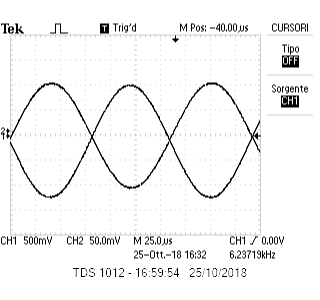
\includegraphics[scale=0.7]{3_1.png}
	\caption{Inversione di fase tra ingresso e uscita} 
	\end{figure}
		
\end{document}